Suspending the optics is one of the most complicated parts of the experiment.
The optics are constructed as discs with roughly 76 mm (3 inch) diameters. 
They are suspended from modified Small Optics Suspensions (SOSs) and controlled with Optical Sensing Electro-Magnets (OSEMs).

\section{Input coupler}

The input coupler (see fig \ref{fig:inputcoupler}) is designed to hold three mirrors at specific positions and angles. The mirrors are 0.5 inches in diameter with 7.5 cm RoC. They are mounted in an approximately 300 gram aluminum disk.
The central mirror forms the straight cavity with the end mirror, while the two mirrors on the side are part of the folded cavity. 
The angle and, to a lesser degree, z position of the two side mirrors are adjustable using set screws. 
 
For each of the adjustable mirrors, set screws push on the bevel of the back surface of the mirror. 
The mirror is held in place by a Teflon tube placed on the front side of the mirror, which is in turn clamped down with springs on screws.
This gives us the flexibility to adjust for manufacturing defects and to adjust the beam separation on the end mirror after construction.

Tapped screws in the top and bottom allow for precision correction of the center of mass of the mass after suspension.
The mirrors are shifted laterally to make the mirrors fit inside the 3.0 inch diameter of the aluminum mass.

The design concerns governing the placement of the holes include the separation of the beams, the angle of the folded cavity, and the desired lengths of the two cavities. 

\begin{figure}[hp]
	\centering
		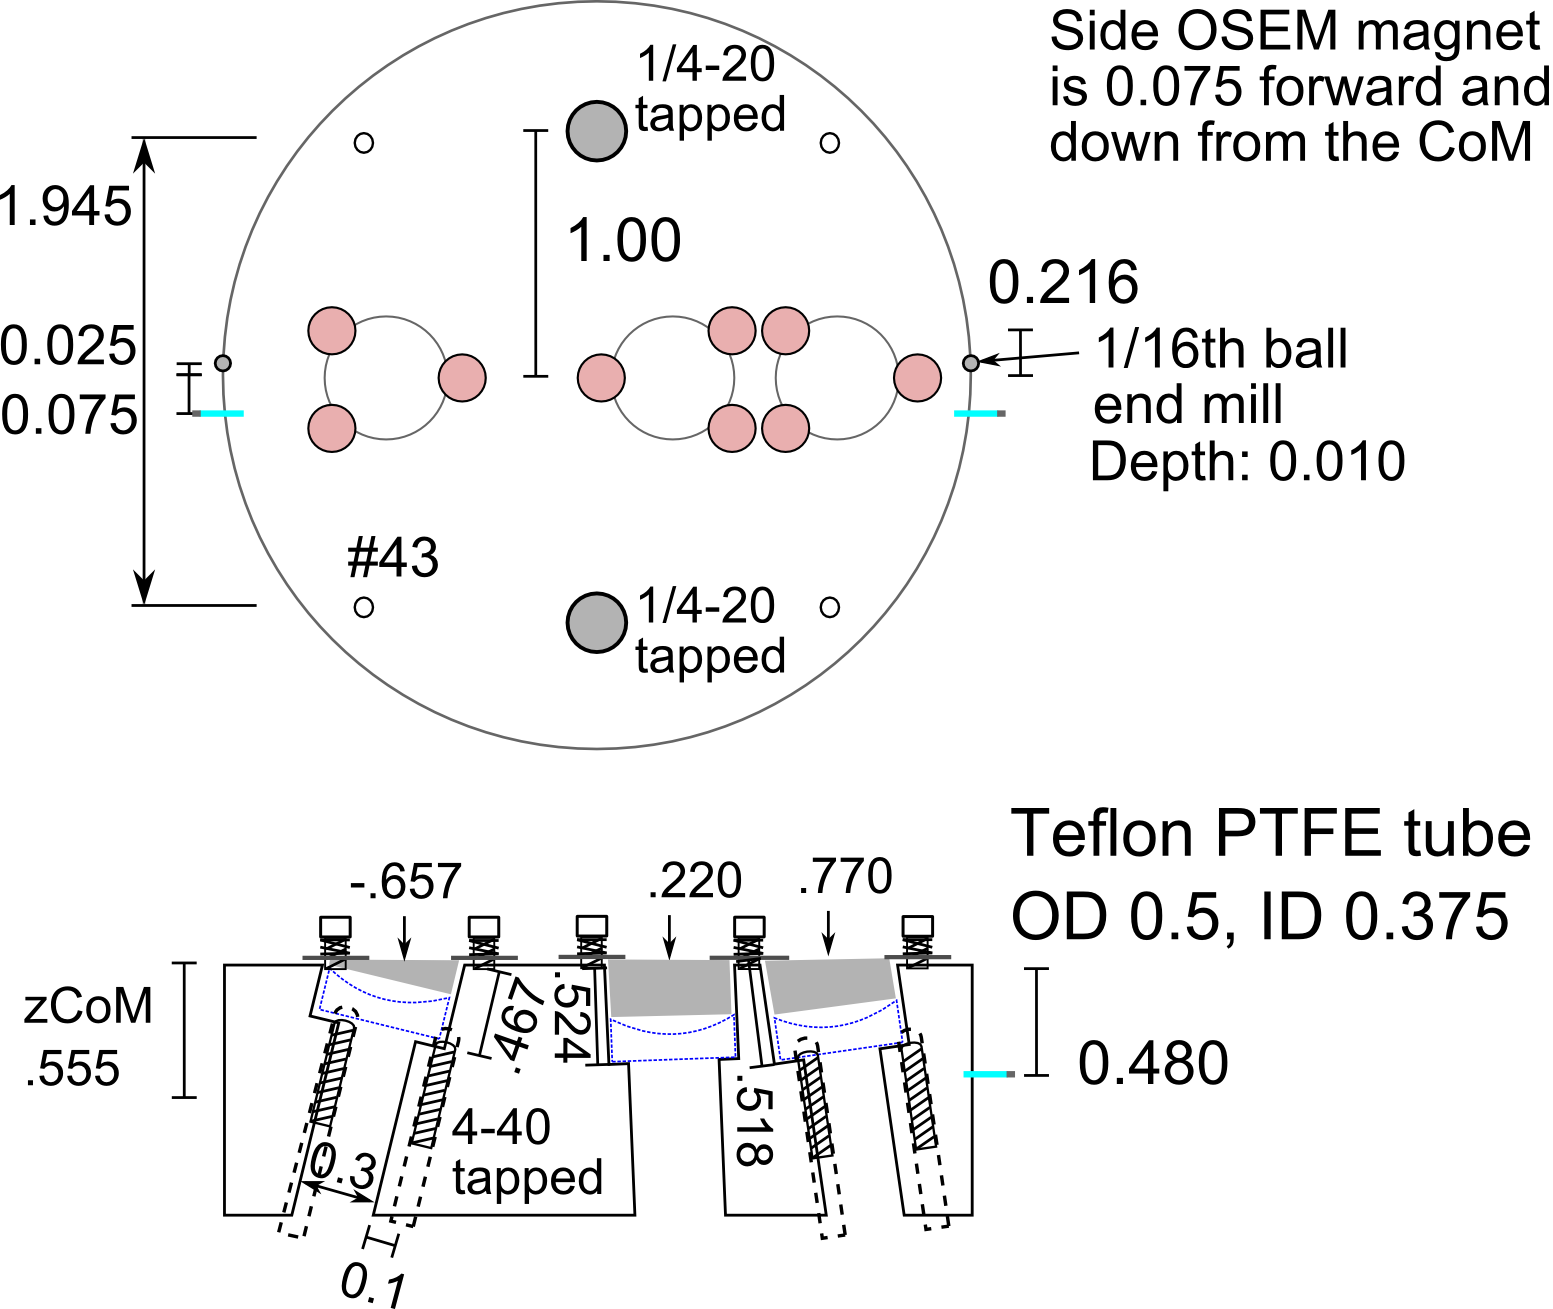
\includegraphics[width=.9\textwidth]{figures/suspensions/inputcoupler.png}
	\caption[Input coupler]{The input coupler for the cavity. Three 0.5 inch diameter mirrors with 7.5 cm RoC are held at specific angles inside an aluminum disk. The two side mirrors are adjustable using set screws, while the central mirror is fixed.}
	\label{fig:inputcoupler}
\end{figure}
 
\section{End mirror}

The end mirror has a diameter of 0.305 inches, a radius of curvature of 5 cm, and a mass of 0.4 grams. It is suspended by glass fibers from a steel ring, which is in turned suspended from a modified SOS. The suspension is pictured in \ref{fig:smallmirrorpic}.

The fibers are manufactured by cold welding a fused silica rod onto a mirror blank, creating a nub, then pulling a fiber off it, to a length of about 1 inch. Once the fiber cools, we break the cold weld. This leaves us with a nub attached to a fiber, which is in turn attached to a silica rod. The silica rod is glued into an aluminum block, which is screwed down to the steel ring. The nubs are then glued to the actual mirror using Optocast 3553. Because the nubs were created on a mirror blank with the same diameter, the volume of glue required is minimized, reducing the thermal noise effects of the glue joint. After gluing on all three fibers, the fibers are tensioned to raise the resonance of the position mode to the desired frequency.

\begin{figure}[htbp]
	\centering
		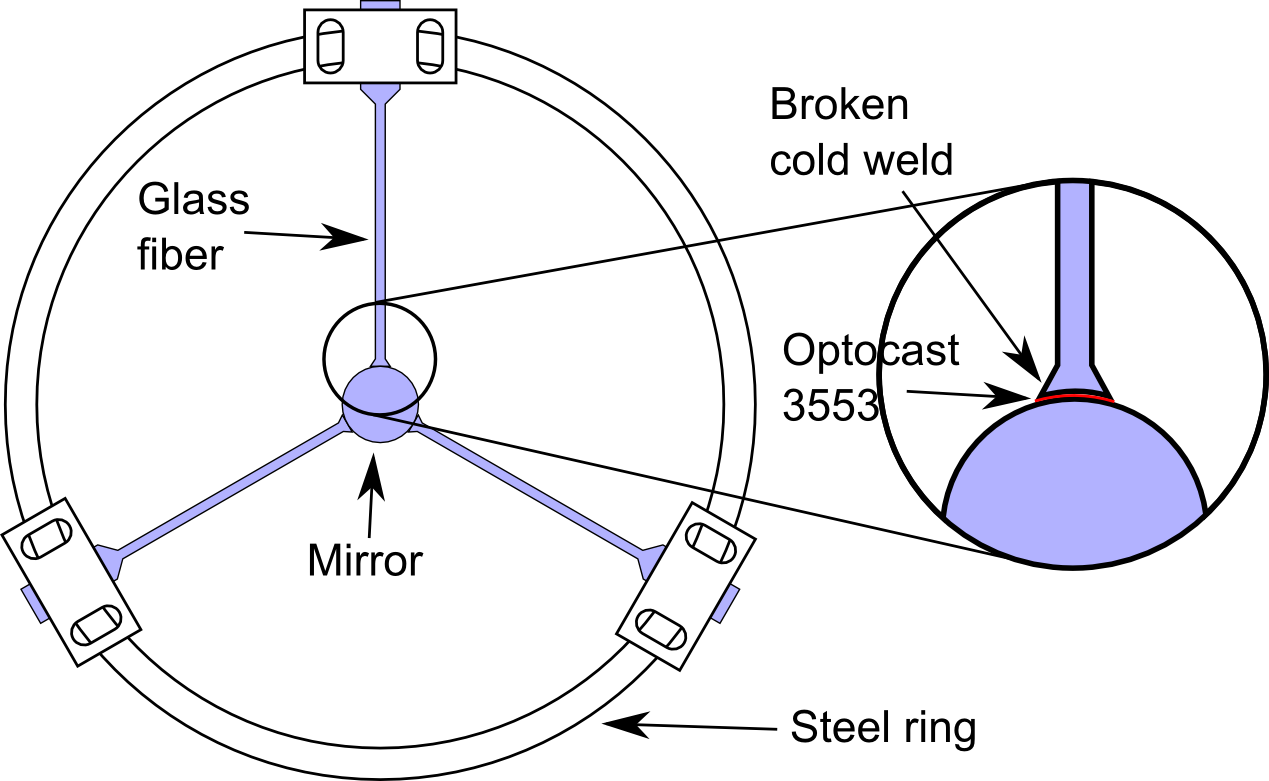
\includegraphics[width=.9\textwidth]{figures/suspensions/smallmass2.png}
	\caption[End mass suspension]{End mass suspension. A 0.4 gram mirror is suspended from a steel ring using glass fibers.}
	\label{fig:smallmassdiagram}
\end{figure}




\section{Blade Springs}
%This is a partial procedure that we have adopted to design a vertical isolation system for a large platform
%used to host the Small Optic Suspensions (SOS) that support our Trap-Cavity. The platform is an aluminum disk with two SOS structures and counterweights, totaling 75 Kg, which will
%be suspended with 3 wires, each attached to a blade spring in order to increase vertical isolation. Fig.\ref{fig:topplate} shows the top plate with its blade springs. The clamp bases will be cut out in order to make them fit on to the plate. 

%\begin{figure}[ht]		
%\centering
%\includegraphics[width=7cm]{topplate.png}
	%\caption{\emph{View of the top plate from below.}}
	%\label{fig:topplate}
%\end{figure}

%We want a relatively low bounce mode frequency, less than 1Hz, with a minimized coupling
%of the vertical motion into the longitudinal one. This requires adjusting dimensional parameters in order to keep the stress under the allowed limit of the material that we are going to use.
This is a discussion of the relevant physics to the construction of blade spring suspensions for a small optics suspension.

This theoretical parts of the paper are based primarily on the notes posted in the DCC
\footnote{https://dcc.ligo.org/LIGO-T030285}.

\subsection{A little theory}
\label{sec:theory}

\begin{figure}[ht]		
\centering
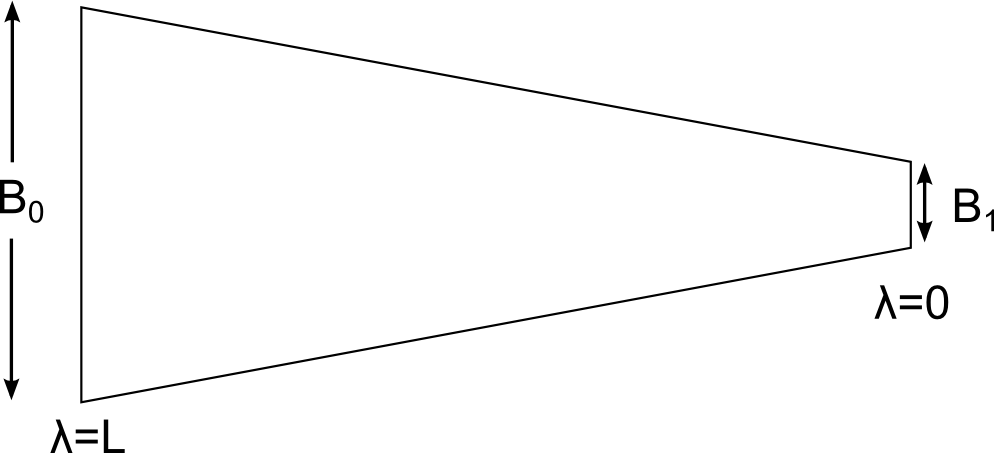
\includegraphics[width=7cm]{figures/suspensions/bladeWidth.png}
	\caption[Blade springs]{Profile drawing of a deflected blade spring. R is the radius of the circle described by the blade spring
	when it is under stress. L is the length of the blade, $b_0$ is the large base and $b_1$ is the small base. $\lambda$ is the distance along the blade}
	\label{fig:bladeIllustration}
\end{figure}

The paper gives the general formula for an elastic beam under a load (see Rourke's formulas for stress and strain, eq. 8.1-4):

\begin{eqnarray}
\frac{E}{R(\lambda)} = \frac{M(\lambda)}{I(\lambda)}
\label{eq:R}
\end{eqnarray}
 
Here $\lambda$ is the distance along the blade (with the $\lambda=0$ at the tip), $E$ is the Young's modulus, $R$ is the radius of curvature at $\lambda$, $I$ is the area moment of inertia at $\lambda$, and $M$ is the bending moment at $\lambda$, expressed as: 

\begin{eqnarray}
M = m g \lambda
\label{eq:M}
\end{eqnarray}

where m is mass supported, g is $9.81 \mbox{m/s}^2$.

$b = b_1+(b_0-b_1) \frac{\lambda}{L}$ is the width between $\lambda=0$ ($b=b_1$) and $\lambda=L$ ($b=b_0$) (see figure \ref{fig:bladeIllustration}) so

\begin{eqnarray}
I = \frac{b t^3}{12} = (b_0-b_1)\frac{t^3}{12} \frac{\lambda}{L}+b_1\frac{t^3}{12}
\label{eq:I1}
\end{eqnarray}


where $t$ is the thickness of the blade and $L$ is the blade length.  If we consider the blade to be triangular ( $b_1=0$), $I$ becomes

\begin{eqnarray}
I = \frac{b_0t^3}{12} \frac{\lambda}{L}
\label{eq:Itri}
\end{eqnarray}

Then we see that 

\begin{eqnarray}
\frac{E}{R(\lambda)} = \frac{M(\lambda)}{I(\lambda)} = 
\frac{m g \lambda}{b_0\frac{t^3}{12} \frac{\lambda}{L}} = 
\frac{12 m g L}{b_0 t^3} \quad \rightarrow \quad R=constant
\label{eq:E/R}
\end{eqnarray}

In other words, R is constant along the blade (the blade profile is circular). We can accomplish this behavior by specifying that the wire is clamped where the end of the `triangle' should be.

%You may have noticed that the calculation is based on an initially flat beam. 
%We attempted to add a cosine term to account for the monting angle, but the predictions were inaccurate.

% However, the modification to the moment calculation for a beam deflection $\theta$ is as simple as accounting for the change in deflection force ($m g \rightarrow m g  \mbox{cos}(\theta)$) (this is assuming that the blade is not compressable in the $\lambda$ direction).

Thus we can, without difficulty, treat a change in force on the spring (for instance by changing the mass) as a change in the radius of curvature of the blade.

%This prediction will obviously break if the end of the spring goes more than one radius below the highest point.

From eq.\ref{eq:E/R} we obtain $R$

\begin{eqnarray}
R(\lambda) = R = \frac{E b_0 t^3}{12 m g L}
%R(\lambda) = R = \frac{E b_0 t^3}{12 m g L \mbox{cos}(\theta)}
\label{eq:Rend}
\end{eqnarray}

From eq.{\ref{eq:Rend}} we can obtain the bounce mode frequency $f_b$

\begin{eqnarray}
f_b = \frac{1}{2\pi}\sqrt{\frac{E b_0 t^3}{6 m L^3}}
%f_b = \frac{1}{2\pi}\sqrt{\frac{E b_0 t^3}{6 m L^3 \mbox{cos}(\theta)}}
\label{eq:fb}
\end{eqnarray}

and the maximum stress in the blade as:

\begin{eqnarray}
\sigma = \frac{6 m g L}{ b_0 t^2};
%\sigma = \frac{6 m g \mbox{cos}(\theta)L}{ b_0 t^2};
\label{eq:stress}
\end{eqnarray}

We can use equation \ref{eq:stress}, solved for $b_0$, to simplify equation \ref{eq:fb}, thus

\begin{eqnarray}
f_b = \frac{1}{2\pi}\sqrt{\frac{E g t}{L^2 \sigma}}
\label{eq:fb2}
\end{eqnarray}

Given a target stress $\sigma$, a target bounce frequency $f_b$, and a length limit $L$ based on the chamber dimensions, we can determine the proper thickness $t$ for the blade.

If we manipulate equations \ref{eq:fb2} and \ref{eq:stress}, we get

\begin{eqnarray}
t = \frac{(2 pi f_b L)^2 \sigma}{E g} = \sqrt{\frac{6 m g L}{ b_0 \sigma}}
%t = \frac{(2 pi f_b L)^2 \sigma}{E g} = \sqrt{\frac{6 m g \mbox{cos}(\theta)L}{ b_0 \sigma}}
\label{eq:thickness}
\end{eqnarray}

This equation gives the minimum requirement to make a blade spring.

% We are left with two related parameters, $\theta$ and $b_0$ which can be written as follow from eq:\ref{eq:stress} eq.\ref{eq:thickness}:  
% 
% \begin{eqnarray}
% \frac{b0}{cos\Theta}=\frac{6mgL}{\sigma t^2}
% \label{eq:b0cos}
% \end{eqnarray}
% 
% We must adjust both, maintaining the constant thickness, to minimize the coupling of vertical motion to horizontal motion at the tip of the blade.  To do this, we plot the blade profile with small variations to the supported mass, simulating a vertical force, and find the mounting angle with the minimum horizontal fluctuation (effective length $z_{max}$ fluctuation) for the supported mass:
% % (See figures \ref{fig:massvlen}):

%\begin{figure}[ht]		
%\centering
%\includegraphics[width=400pt]{massvlen.png}
	%\caption{\emph{Effective blade length as a function of mass applied. By recalculating the radius of curvature with varying masses, we can simulate the effect of applying a vertical force to the payload. }}
	%\label{fig:massvlen}
%\end{figure}


% \subsection{Blade profile plot}
% %$f_b$ is the predicted bounce mode frequency for the blade spring, loaded with 25 kg.
% 
% We can plot the blade profile by changing to a basis $\phi = \frac{\lambda}{R}+\phi_i$ where $\phi_i = \pi/2 -\theta$ is the initial $\phi$ such that the initial blade spring angle is $\theta$, then we can do a parametric plot (see Fig. \ref{fig:bladeIllustration}) with the longitudinal axes $z$ and the vertical axes $y$ defined as following:
% 
% \begin{eqnarray}
% z&=&-R(\mbox{cos}(\phi)-\mbox{cos}(\phi_i))\\
% y &=& R(\mbox{sin}(\phi)-\mbox{sin}(\phi_i))
% \label{eq:yzparam}
% \end{eqnarray}
% 
% Using this method, we can easily predict important blade measurements such as effective length, maximum blade height, and tip height.
%  %$z=-R(\mbox{cos}(\phi)-\mbox{cos}(\phi_i))$ and $y = R(\mbox{sin}(\phi)-\mbox{sin}(\phi_i))$ as (See Fig.\ref{fig:bladeIllustration}) . 
%We can now look at the blade spring profile when different weights are attached to it. We notice from Fig.\ref{fig:bladeprofilen} the changes in height at different applied forces and at a fixed initial angle. \tcb{is this plot correct?}

%\tcb{From this plot, we can determine the maximum height, the effective length, and the lateral change in the tip due to vertical force fluctuations.}

%\begin{figure}[ht]
	%\centering
		%\includegraphics[width=300pt]{bladeprofile.png}
	%\caption{\emph{Blade profile for $\theta = 49^\circ$.}}
	%\label{fig:bladeprofile}
%\end{figure}

 
% and \ref{fig:heightvlen}.
%
%At the peak of the curves, you can see that for small variations in mass, the slope goes to zero.
%
%%%%%%  MATERIALS  %%%%%%%%%%%%%%%%%%%%%%%%%%%%%%%%%%%%%%%%%%%%%%%%%%
\subsection{Materials}

The LIGO-recommended material is ``maraging'' steel (sometimes known by the tradename Vascomax), which is easy to machine, but becomes incredibly hard when baked.  One drawback of this material is that it can corrode over time.  To combat this, LIGO recommends putting a nickel plating on the blades \footnote{https://dcc.ligo.org/LIGO-E0900023}.  The hardness of the final product is the primary reason it is used.  This material is difficult and expensive (best offer was \$1200 for six blade's worth) to buy in small quantities.  

As an alternative, we are considering ``full hardened'' 301 stainless steel.  It is a factor of about 2.5 weaker than the maraging steel, but we have have found that workable solutions exist.

A third alternative is 17-4 precipitation hardened (PH) stainless.  This material is similar to maraging steel in that it becomes harder when you bake it.  Baking at 900 F for one hour results in a yield strength of 200000 psi = 1379 MPa.  Baking longer or at a higher temperature makes the material a bit sorfter, but this behavior is understood and fairly error-tolerant \footnote{http://www.aksteel.com/pdf/markets\_products/stainless/precipitation/17-4\_PH\_Data\_Bulletin.pdf}

One more alternative which LIGO uses for the small blade springs is 304 stainless (yield strength of 200 MPa) because the expected strain in the small blades is about 80 MPa.

For comparison, McMaster has details of many of the metals that are available \footnote{http://www.mcmaster.com/library/20121105/8984KAC.pdf}. All of the metals we are considering are on the LIGO vacuum compatible materials list\footnote{https://dcc.ligo.org/LIGO-E960050}.

When we are determining the maximum amount of stress that the blade can withstand before deforming, we typically use the yield strength.  This is the amount of stress that causes the metal to deform by 0.2\%.  We have chosen as a target strain 60\% of the yield strength.

One LIGO document \footnote{https://dcc.ligo.org/LIGO-T0900324} adds a factor related to the Poisson's Ratio to the Young's Modulus which effectively increases the strain.  This is attributed to a change in the strain of the material due to bending.  Our predictions seem to work better with this factor removed, but we have chosen to keep the factor for the moment because it represents the `worst case' scenerio.  



\begin{table}[ht]
	\centering
		\begin{tabular}{ l | l | l | l | l }
			Steel & E (GPa) & E (psi) & $\sigma_{max}$ (MPa)  & $\sigma_{max}$ (PSI) \\ \hline
			C350 Maraging & 200 & $29\times10^6$ & 2344 & $34\times10^4$ \\ \hline
			301 Stainless & 193 & $28\times10^6$ & 965 & $14\times10^4$ \\ \hline
			17-4 PH Stainless & 196.5 & $28.5\times10^6$ & 1379 & $20\times10^4$\\ \hline
			304 Stainless &  193 & $28\times10^6$ & 207 & $3\times10^4$
		\end{tabular}
	\caption{Characteristics of proposed materials.}
	\label{tab:materials}
\end{table}

\subsection{Blade spring design}

Criteria for the design following the section \ref{sec:theory}:

\begin{enumerate}
	\item Maintain safe levels $\leq 80\%$ of material stress limits:
	$\sigma\leq0.8\sigma_{max}$.
	\item Blades must be mounted on top of the existing suspensions; smaller is better. 
%  \item All parts must fit within the area of the 27 inch diameter top plate in the bell jar. The length $L$ of the blade springs is fixed at 19''; when under load the bending will reduce the effective length.
  \item Choose a `small' (within reason) bounce mode frequency (This determines $t$). 
  % \item Choose a `small' (within reason) bounce mode frequency (from here we get $t$). 
	\item Minimize vertical to horizontal coupling, looking at the effective length $z_{max}$ as a function of different loads and angles. We could adjust the weight for a given angle or at fixed weight we adjust the angle. The latter is our way to go.
	
\end{enumerate}
%Using equations from \ref{eq:Rend} to \ref{eq:thickness} we have found parameters that satisfy the criteria.  We are using 17-4 stainless steel.  
%The maximum stress of this design is only 60\% of the expected yield strength of the material.  
%This gives us more leeway with the construction and reduces the chance of failure sue to improper baking.  
%The final design schematic is shown in figure \ref{fig:bladeschematic}

%We have two possibilities, one more aggressive in pursuing the lowest bounce mode frequency than the other.  Both utilise 301 stainless steel.

%\subsection*{Proposal 1: $f_b$= 0.9 Hz}
%
%\begin{table}[ht]
%\centering
%\begin{tabular}{ l | l | l }
%\bf{Parameter}& \bf{Metric} & \bf{Imperial} \\ \hline
%Blade length, $L$ & 48.3 cm & 19.0 in \\ \hline
%Blade base width, $b_0$ & 7.9 cm & 3.13 in \\ \hline
%Blade thickness, $t$ & 2.76 mm & 1088 in \\ \hline
%Mounting angle, $\theta$ & 0.850 rad & $48.69^\circ$ \\ \hline
%Supported mass, $m$ & 25 kg & 55 lbs
%\end{tabular}
%\caption{Proposed blade parameters}
%\label{tab:params09}
%\end{table}
%
%\begin{table}[ht]
%\centering
%\begin{tabular}{ l | l | l}
%\bf{Result} & \bf{Metric} & \bf{Imperial} \\ \hline
%Bounce Frequency, $f_b$ & 0.9 Hz \\ \hline
%Max height & 12.9 cm & 5.08 in \\ \hline
%Tip height & 9.6 cm & 3.78 in \\ \hline
%Effective length & 44.0 cm & 17.34 \\ \hline
%Maximum Stress, $\sigma$ & 772 MPa & 112000 PSI
%\end{tabular}
%\caption{Characteristics of proposed blade design}
%\label{tab:results09}
%\end{table}
%\subsection*{Proposal 2: $f_b$= 0.8 Hz}
%
%\begin{table}[H]
%\centering
%\begin{tabular}{ l | l | l }
%\bf{Parameter} & \bf{Metric} & \bf{Imperial} \\ \hline
%Blade length, $L$ & 48.3 cm & 19.0 in \\ \hline
%Blade base width, $b_0$ & 9.1 cm & 3.59 in \\ \hline
%Blade thickness, $t$ & 2.18 mm & 0.0860 in \\ \hline
%Mounting angle, $\theta$ & 1.078 rad & $61.75^\circ$ \\ \hline
%Supported mass, $m$ & 25 kg & 55 lbs
%\end{tabular}
%\caption{Proposed blade parameters}
%\label{tab:params08}
%\end{table}
%
%\begin{table}[H]
%\centering
%\begin{tabular}{ l | l | l}
%\bf{Result} & \bf{Metric} & \bf{Imperial} \\ \hline
%Bounce Frequency, $f_b$ & 0.8 Hz \\ \hline
%Max height & 15.8 cm & 6.22 in \\ \hline
%Tip height & 11.7 cm & 4.59 in \\ \hline
%Effective length & 41.6 cm & 16.38 \\ \hline
%Maximum Stress, $\sigma$ & 772 MPa & 112000 PSI
%\end{tabular}
%\caption{Characteristics of proposed blade design}
%\label{tab:results08}
%\end{table}
%\newpage
%\subsection*{Proposal: Large Springs $f_b$= 0.9 Hz}
%
%\begin{table}[ht]
%\centering
%\begin{tabular}{ l | l | l }
%\bf{Parameter}& \bf{Metric} & \bf{Imperial} \\ \hline
%Blade length, $L$ & 48.3 cm & 19.0 in \\ \hline
%Blade base width, $b_0$ & 7.8 cm & 3.07 in \\ \hline
%Blade thickness, $t$ & 2.76 mm & 1088 in \\ \hline
%Mounting angle, $\theta$ & 0.849 rad & $48.67^\circ$ \\ \hline
%Supported mass, $m$ & 25 kg & 55 lbs\\\\
%\bf{Result} & \bf{Metric} & \bf{Imperial} \\ \hline
%Bounce Frequency, $f_b$ & 0.9 Hz \\ \hline
%Max height & 12.9 cm & 5.08 in \\ \hline
%Tip height & 9.6 cm & 3.77 in \\ \hline
%Effective length & 44.0 cm & 17.34 \\ \hline
%Maximum Stress, $\sigma$ & 786 MPa & 114000 PSI
%\end{tabular}
%\caption{Characteristics of proposed blade design}
%\label{tab:results09}
%\end{table}


%\subsection*{Proposal 2: $f_b$= 0.8 Hz}


%There are distinct advantages for each proposal.  The higher maximum blade height of the 0.8 Hz blade will result in a longer pedestal for the clamp (to lower the mounting point), lowering the resonances of the pedestal (but we expect they will still be very high).  The shorter effective length of the 0.8 Hz blade will make our setup a bit more flexible.  The larger radius of curvature of the 0.9 Hz blade will reduce the horizontal-vertical coupling. 
%
%The mounting angle may or may not be an issue, depending on how well our simulations work.  The frequency difference actually makes very little difference for anything over 5 Hz.

%\newpage



%
%\subsection{Couplings}
%
%With a vertical seismic noise RMS motion of $10^{-7}$ m, we could expect that to be coupled to the `twist' mode of the optical table (because the springs all point in the same direction around the center of the table).
%
%If properly aligned (parameters properly chosen), we are in a situation where there is a minimised coupling between the vertical and the longitudinal motion. The horizontal motion is described by $z$ and the vertical motion is described by the tip motion along $y$ (see Fig.\ref{fig:heightvlen}).
%%
%%\begin{figure}[htp]		
%%\centering
%%\includegraphics[width=350pt]{heightvlen.png}
	%%\caption{\emph{Effective blade length as a function of blade tip height. A vertical motion of $1\,$mm longitudinal motion coupling
	%%of the order of a micron.}}
	%%\label{fig:heightvlen}
%%\end{figure}
%
%
%We could expect couplings of up to $4\times10^-3$ if we are off from that point by a milimeter.  Thus a vertical RMS displacement of $10^{-7}$ m could result in a twist RMS displacement of $10^{-10}$ m.  
%Fig.\ref{fig:seismic} shows seismic motion coupled into vertical and longitudinal motions. 
%
%%\begin{figure}[hp]
	%%\centering
		%%\includegraphics[width=400pt]{seisplot.png}
	%%\caption{\emph{Expected seismic motion, taken from David's noise budget. At this level the horizontal coupling (red line)  does not seem to be an issue. }
%%}
	%%\label{fig:seismic}
%%\end{figure}
%
%
%%\begin{figure}[p]
	%%\centering
		%%\includegraphics[width=600pt, angle=90]{blade.png}
	%%\caption{\emph{Design of large blade}}
	%%\label{fig:bladeschematic}
%%\end{figure}
%
%\newpage

\subsection{Small blade}

At the same time, we are designing a similar suspension to be mounted on top of each SOS.  These will be much smaller, but will follow the same design principles.


For the small spring system, our design is very similar to the parameters used in the HAM AUX design for ALIGO \footnote{https://dcc.ligo.org/LIGO-T1000339}  We can use 304 Stainless or 17-4 Stainless with little impact on the final performance.  The maximum stress of this design is only 40\% of the expected yield strength of 304 and much less than that for 17-4.  This gives us more leeway with the construction and reduces the chance of failure due to improper baking.  The final design schematic is shown in figure \ref{fig:babyschematic}.  For the small design we have chosen to neglect the Poisson Ratio factor because the bending is much smaller.  We are motivated to do this by the HAM AUX design mentioned earlier.

\begin{table}[ht]
\centering
\begin{tabular}{ l | l | l }
\bf{Parameter}& \bf{Metric} & \bf{Imperial} \\ \hline
Blade length, $L$ & 7.68 cm & 3.0 in \\ \hline
Blade base width, $b_0$ & 3.3 cm & 1.3 in \\ \hline
Blade thickness, $t$ & 0.51 mm & 0.020 in \\ \hline
Mounting angle, $\theta$ & 0.083 rad & $4.78^\circ$ \\ \hline
Supported mass, $m$ & 0.15 kg & 0.33 lbs\\\\
\bf{Result} & \bf{Metric} & \bf{Imperial} \\ \hline
Bounce Frequency, $f_b$ & 7.19 Hz \\ \hline
Max height & 2 mm & 0.08 in \\ \hline
Tip height & 2 mm & 0.06 in \\ \hline
Effective length & 7.7 cm & 3.0 in \\ \hline
Maximum Stress, $\sigma$ & 81 MPa & 11700 PSI
\end{tabular}
\caption{Characteristics of proposed blade design}
\label{tab:resultsBaby}
\end{table}

\subsection{Coupling}
For the small spring system, we do not need to worry about this coupling because the motion will not couple to the position degree of freedom to first order.  We should note that changing the effective length would result in a change in the yaw mode resonance of the suspended structure, which may be an issue. 



\begin{figure}[hp]
	\centering
		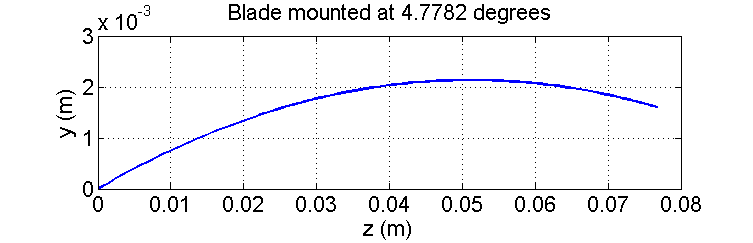
\includegraphics[width=.9\textwidth]{figures/suspensions/babybladeprofile.png}
	\caption[Blade profile for small suspension.]{Expected profile of the small blade supporting 300 grams.}
	\label{fig:babybladeprofile}
\end{figure}





\begin{figure}[p]
	\centering
		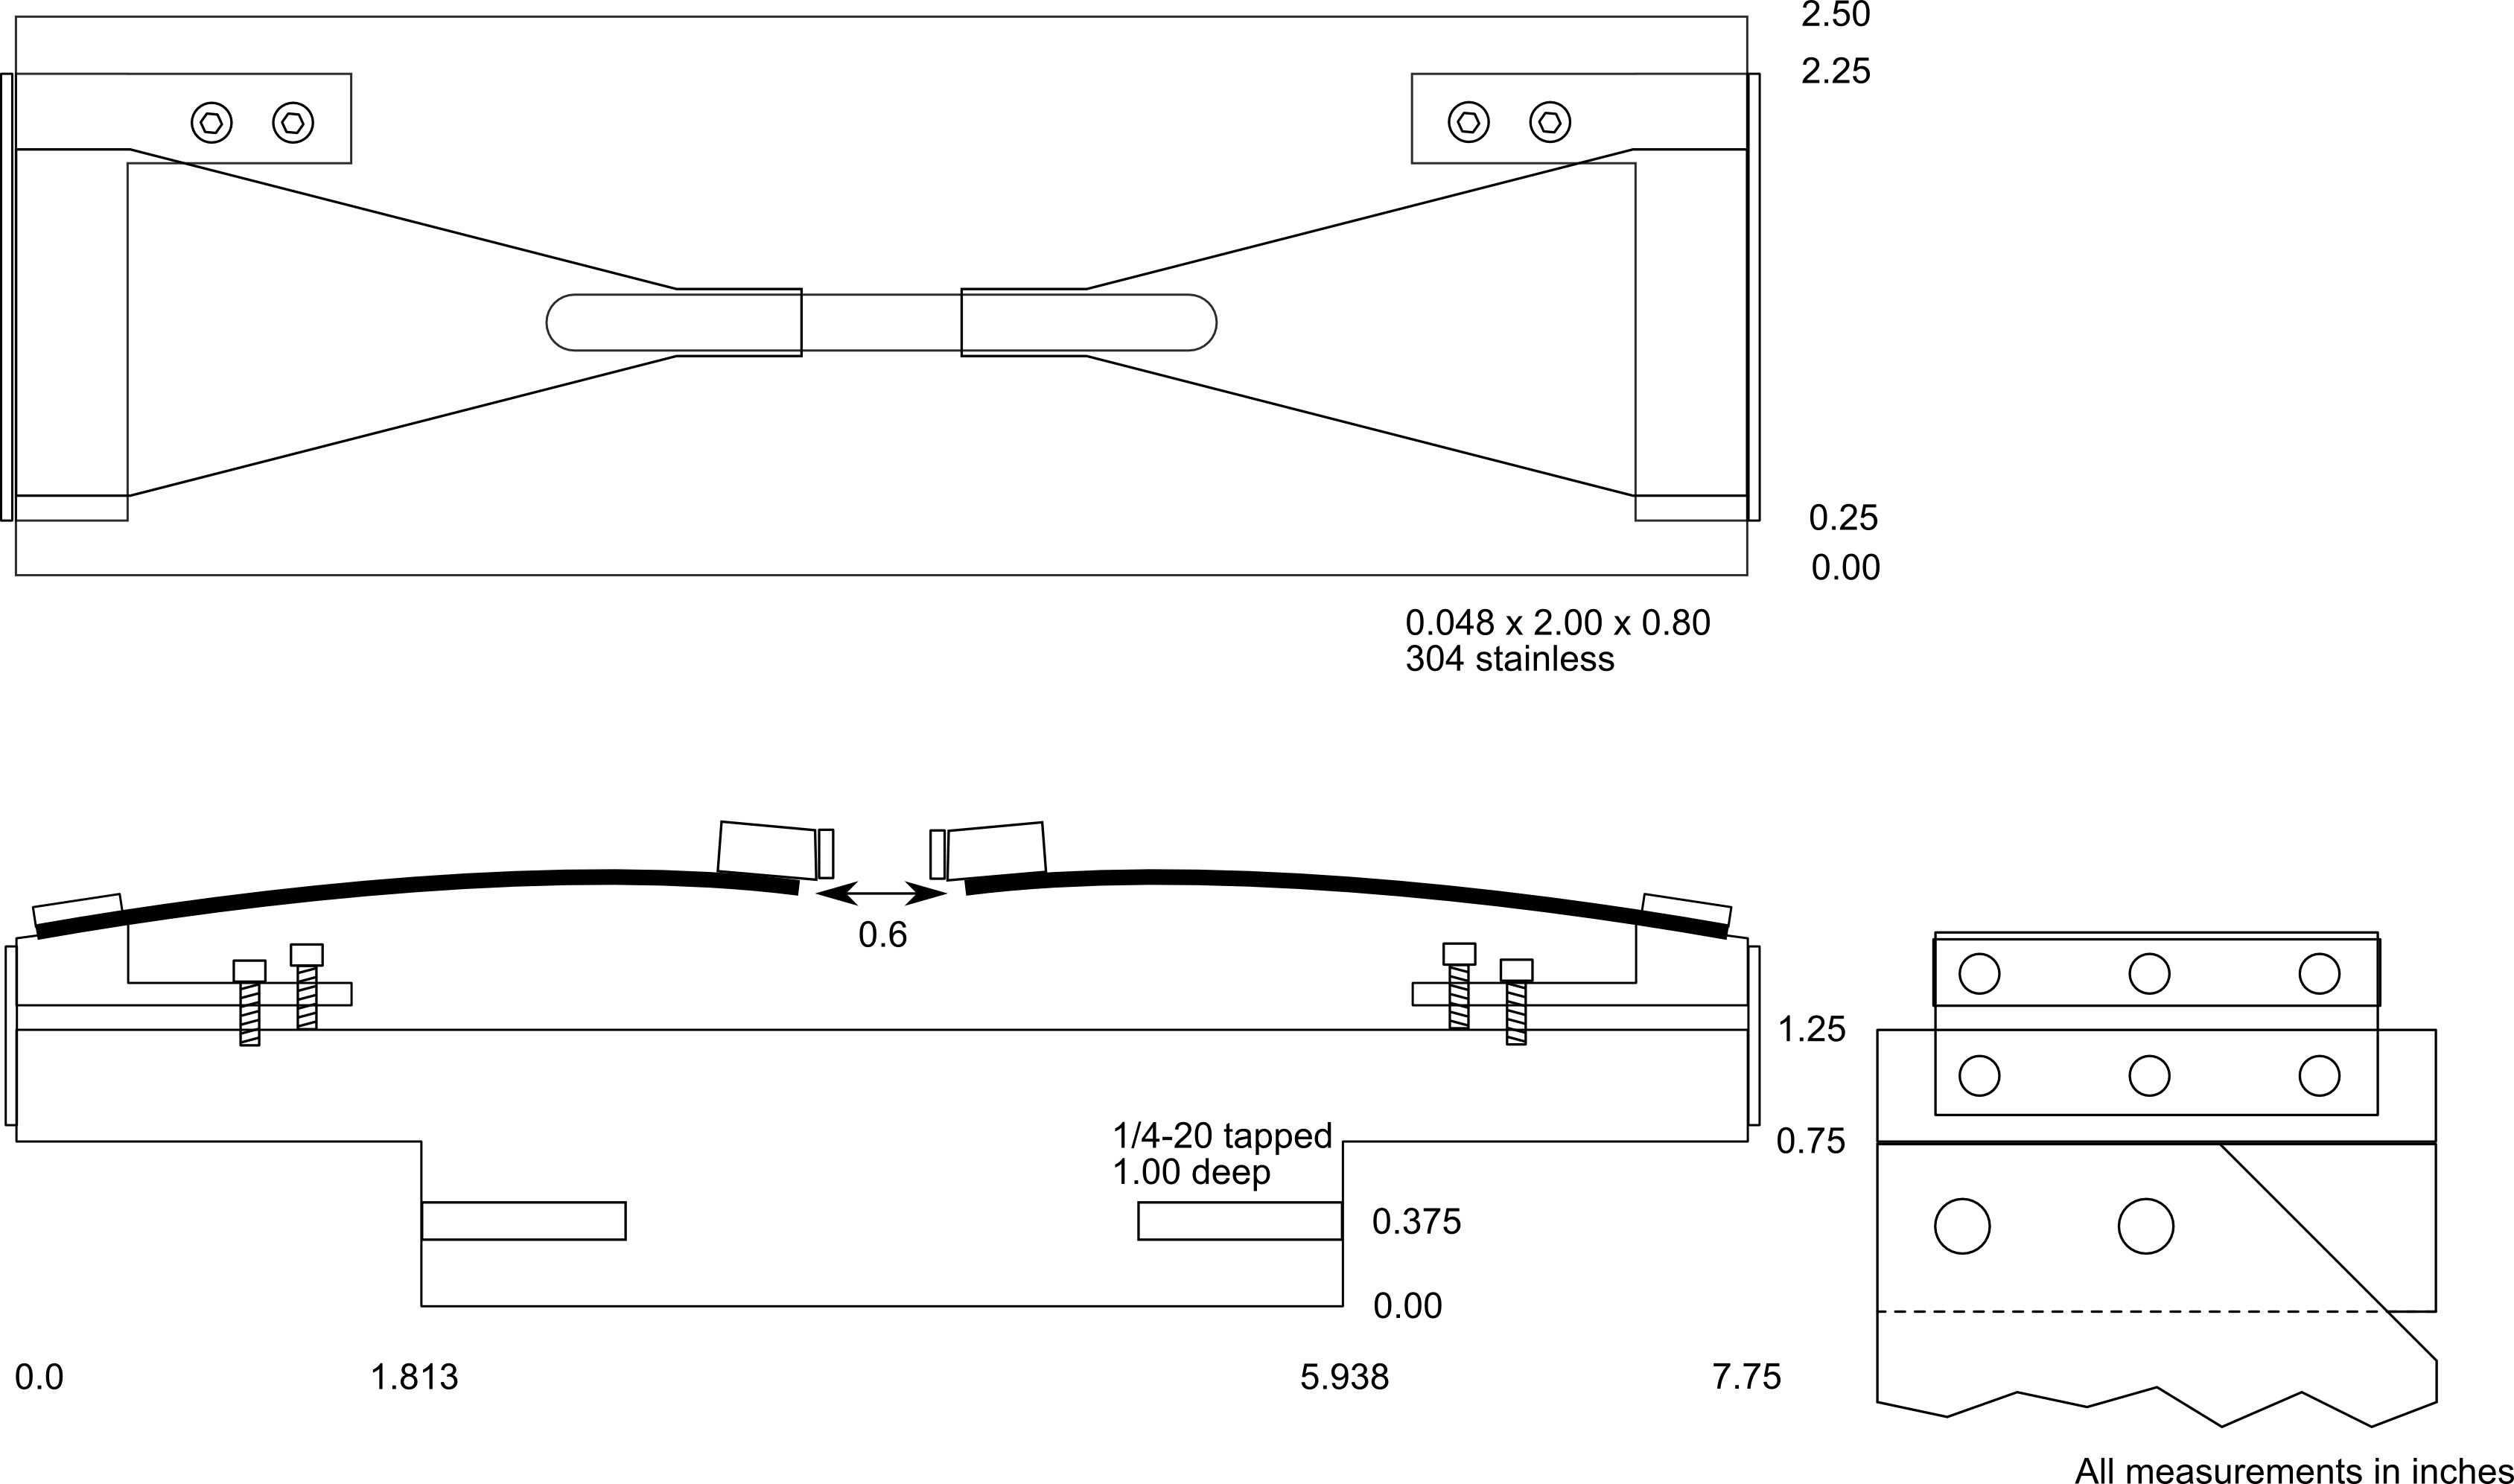
\includegraphics[width=\textwidth, angle=90]{figures/suspensions/bb1.png}
	\caption[Small blade design]{Drawings for the small blade suspension modification to the SOS. The blade angle can be adjusted using the screws. This adjustment was used for fine adjustment of the optic height and rotation.}
	\label{fig:babyschematic}
\end{figure}
\section{OSEM diagonalzation}

To control the mass under vacuum, we use devices called OSEMs (Optical Sensing Electro-Magnets). These are devices (see fig. \ref{fig:osem}) that sense the position of an optic using magnets which are mounted on the optic. The magnet partially blocks light from an LED, so when it moves it causes changes in the voltage out from a photodiode. This signal is sent to the digital system, where it is converted into position, pitch, yaw, and side motion. Each of these degrees of freedom have specific filters applied to them, then the signals are converted back into the five sensor distances. Coils in the OSEM are driven accordingy, controlling the motion of the optic.

\begin{figure}[hp]
	\centering
		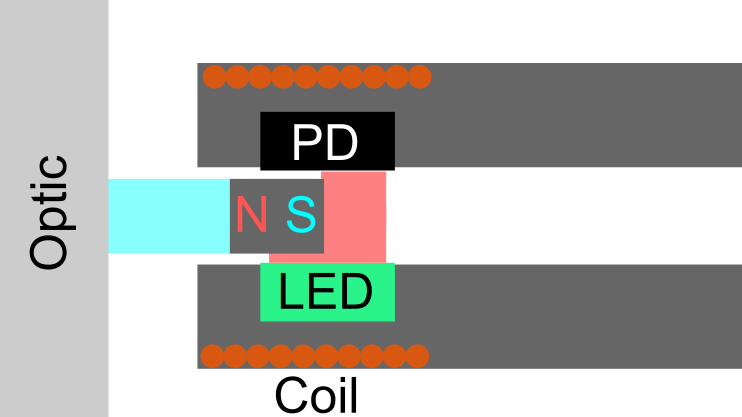
\includegraphics[width=.5\textwidth]{figures/suspensions/OSEM.png}
	\caption[OSEM diagram]{Layout of an Optical Sensing Electro-Magnet (OSEM). Optic motion is sensed when the magnet changes the amount of light from the light emitting diode (LED) that gets to the photodiode (PD). The coils can be driven to move the magnet and thus the optic.}
	\label{fig:osem}
\end{figure}

The hardest part to get right when using OSEMs is to properly diagonalize them so that you can push in the standard degrees of freedom (i.e. position, pitch, yaw, and side). This is accomplished in two steps, along with some sneaky meter-to-radian conversion. 

First, we diagonalize the input matrix. An ideal input matrix should look like table \ref{tab:idealDiag}. The input values are converted to micrometers before they get to this matrix. This matrix then converts the measurements to position and side measurements in $\mu m$ and pitch and yaw measurements in $\mu rad$ (the angular conversion is dependent on the fact that the magnets are mounted in a 4.94 by 4.94 cm square). Thus a change of $1 \mu m$ the upper left (UL) sensor is counted as : $.25 \mu m$ position, $-10.1 \mu rad$ in pitch, $10.1 \mu rad$ in yaw, and no change in side.

\begin{table}[hp]
\centering
\begin{tabular}{| c | c | c |c | c | l}
\bf{UL}& \bf{UR} & \bf{LR}  & \bf{LL} & \bf{SD}\\ \hline
  .25 & .25 & .25 & .25 & 0 &position ($\mu m$)\\
 -10.1 &-10.1 & 10.1 & 10.1 & 0 &pitch ($\mu rad$)\\
  10.1 &-10.1 &-10.1 & 10.1 & 0 &yaw ($\mu rad$)\\
  0 & 0 & 0 & 0 & 1 &side ($\mu m$)\\ \hline
\end{tabular}
\caption[Ideal diagonalization]{Ideal input matrix. The sensor inputs (in $\mu m$) are multiplied by the coefficients to get position of the mass in two directions (position and side) and the orientation of the mass (pitch and side). The coefficient for the angular measurements is calculated from the distance (1.945 in) between the magnets mounted on the mass.}
\label{tab:idealDiag}
\end{table}

However, due to OSEM alignment, machining defects, suspension inaccuracy, etc. the ideal matrix is not the most effective. Thus, we have a method for diagonalizing the matrices.

We drive one OSEM and look at the transfer function between that and all of the other OSEMs. We can determine from this the different modes (pos, pit, and yaw) by looking at the phase differences between the four back OSEMs (UL UR LL LR) at resonances. After this, we orthogonalize based on the coupling of each mode to the five osems. Here we have one interesting note: the position mode that we see is actually the pendulum mode, which is a combination of the pitch and position modes of the mass. The coupling scales inversely with the pendulum length.

\begin{figure}[p]
	\centering
		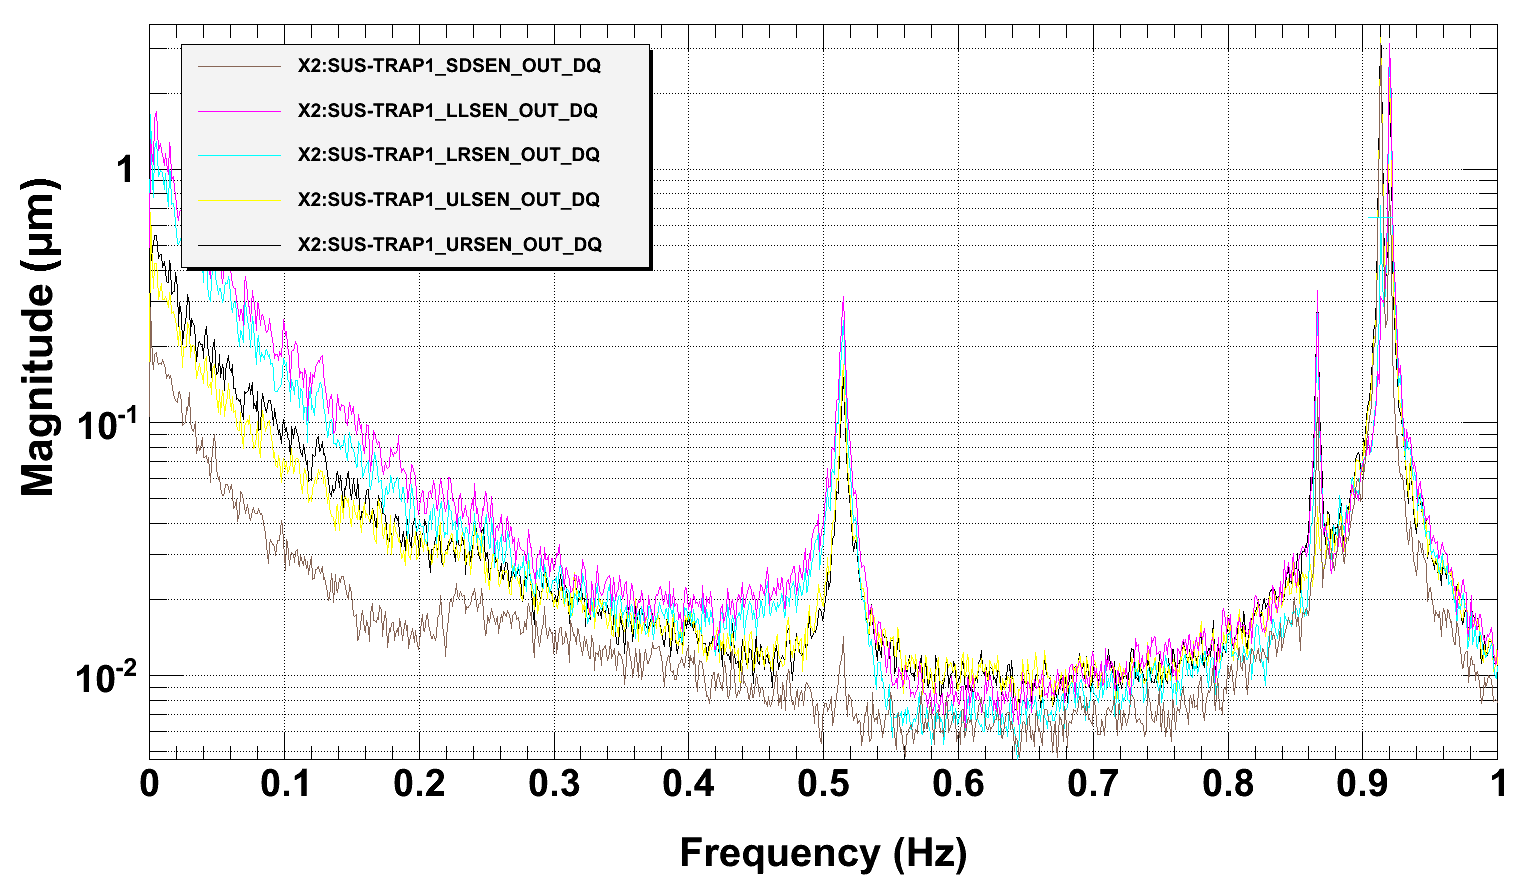
\includegraphics[width=.95\textwidth]{figures/suspensions/trap1spec.png}
	\caption[Input coupler spectrum]{Spectrum showing the modes of the input coupler.  Modes from low to high are: Pitch (0.511 Hz), Yaw (0.866 Hz), Side (0.911 Hz), and Position (0.918 Hz). }
	\label{fig:trap1spec}
\end{figure}


Once we have the input matrix set, we diagonalize the output matrix. We close the loops and drive each degree of freedom with a slow signal, then measure the responses in each of the (properly diagonalized) sensors. We subtract out the drive to the not desired degrees of freedom to determine the output matrix. 
%
%\begin{figure}[p]
	%\centering
	%\caption[Diagonlization noise comparison]{Plot showing the nosie before and after diagonalization}
	%\label{fig:diagNoise}
%\end{figure}
